\documentclass[twocolumn,10pt]{article}
\title{Constructing geometric figures}
\setlength{\columnsep}{20pt} 
\usepackage{amsmath,hyperref,cancel,graphicx}
 \def\shrinkfactor{0.45}
 \usepackage[margin=1.5cm]{geometry}
\usepackage[usenames,dvipsnames]{color}
 
 \newcommand{\blue}[1]{{\color{Blue}#1}} 
 \newcommand{\purple}[1]{{\color{Purple}#1}} 
 \newcommand{\red}[1]{{\color{Red}#1}} 
 \newcommand{\green}[1]{{\color{Green}#1}} 
 \newcommand{\gray}[1]{{\color{Gray}#1}} 
  \newcommand{\pink}[1]{{\color{Magenta}#1}}   


\begin{document}
\maketitle



\section{\href{https://www.khanacademy.org/devadmin/content/items/x0341d7bd2961f8ac}{x0341d7bd2961f8ac}}

\noindent
**How many quadrilaterals can be drawn with four obtuse angles?**

\paragraph{Ans} 

\fbox{ None

}

 Only one

More than one



\paragraph{Hint 1}A quadrilateral is a plane figure with four straight sides and four angles. In general, all four angles of a quadrilateral sum to $\pink{360^\circ}$.

Obtuse angles are more than $\blue{{90}^\circ}$ and less than $\blue{{180}^\circ}$.  Let's start by trying to draw a quadrilateral with four obtuse angles

\paragraph{Hint 2}We can draw a quadrilateral with at most two obtuse angles.  


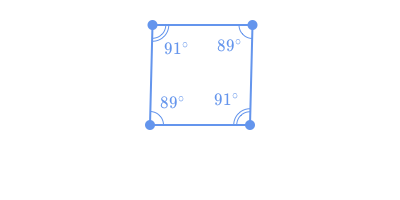
\includegraphics[scale=\shrinkfactor]{figures/3fcc8a0717d83f7b047263027d42633407987b91.png}

\paragraph{Hint 3}Given the conditions, no quadrilaterals can be drawn.



\medskip
\noindent
\textbf{Tags:} {\footnotesize CC.7.G.A.2, Constructing geometric figures}\\
\textbf{Version:} 8bf1a7c0.. 2013-10-21
\smallskip\hrule





\section{\href{https://www.khanacademy.org/devadmin/content/items/x0a4cebeb1feb4470}{x0a4cebeb1feb4470}}

\noindent
**How many quadrilaterals can be drawn with four acute angles?**

\paragraph{Ans} 

\fbox{ None

}

 Only one

More than one



\paragraph{Hint 1}A quadrilateral is a plane figure with four straight sides and four angles. In general, all four angles of a quadrilateral sum to $\pink{360^\circ}$.

Acute angles are less than $\blue{{90}^\circ}$.  Let's start by trying to draw a quadrilateral with four acute angles.

\paragraph{Hint 2}We can draw a quadrilateral with at most two acute angles.  


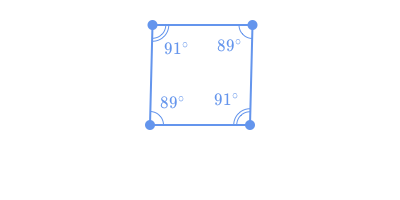
\includegraphics[scale=\shrinkfactor]{figures/3fcc8a0717d83f7b047263027d42633407987b91.png}

\paragraph{Hint 3}Given the conditions, no quadrilaterals can be drawn.



\medskip
\noindent
\textbf{Tags:} {\footnotesize CC.7.G.A.2, Constructing geometric figures}\\
\textbf{Version:} e80a1b6a.. 2013-10-21
\smallskip\hrule





\section{\href{https://www.khanacademy.org/devadmin/content/items/x1e00032cb06e0d1d}{x1e00032cb06e0d1d}}

\noindent
**Draw an isosceles trapezoid with two sets of angles $59^\circ$ and $121^\circ$ and a set of bases of length $a$ and $2.5a$ where $a$ is any positive number.** 

**With these conditions, is the trapezoid unique?**
[[? interactive-graph 1]]

\paragraph{Ans} 

Yes

\fbox{ No

}

 

\paragraph{Hint 1}An isosceles trapezoid has four sides with two parallel bases and two nonparallel sides equal in length.

Let's choose any positive value for $\blue{a}$ and draw a trapezoid given the conditions.

\paragraph{Hint 2}If $\blue{a}=\blue{4}$, then lets draw parallel bases of length $\blue4$ and length $\blue{10}$. Let's adjust the height of the trapezoid until we draw $\blue{59^\circ}$ and $\blue{121^\circ}$ angles and have nonparallel sides equal in length.


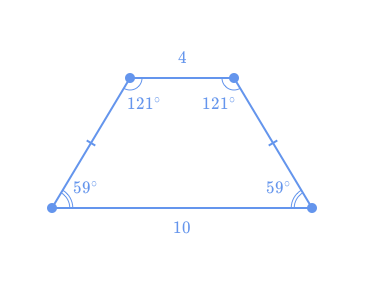
\includegraphics[scale=\shrinkfactor]{figures/3fc1a3de04ae5beee01136dbc98446947a8f58f8.png}

\paragraph{Hint 3}We know only the measures of the four angles, do not know the measures of the nonparallel sides, and can choose any positive value for $\blue{a}$. We can draw more than one isosceles trapezoid of the same shape but different size.

\paragraph{Hint 4}With the given conditions, the isosceles trapezoid is not unique.


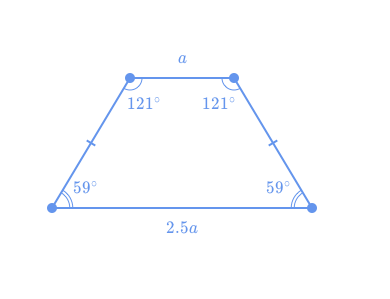
\includegraphics[scale=\shrinkfactor]{figures/249bf35a334a6b61176c6935259fb138330fc7bb.png}



\medskip
\noindent
\textbf{Tags:} {\footnotesize CC.7.G.A.2, Constructing geometric figures}\\
\textbf{Version:} fc3cd11f.. 2013-10-22
\smallskip\hrule





\section{\href{https://www.khanacademy.org/devadmin/content/items/x2e4bec2b838f401f}{x2e4bec2b838f401f}}

\noindent
**Draw a quadrilateral with a set of $104^\circ$ angles, a set of $76^\circ$ angles, a set of sides length $6$, and a set of sides length $5.2$.** 

**Is there a unique quadrilateral that satisfies the given conditions?**
[[? interactive-graph 1]]

\paragraph{Ans} 

\fbox{ Yes

}

 No



\paragraph{Hint 1}A quadrilateral has four straight sides and four angles. Since we have two sets of equal angles and two sets of equal sides sides, we have a parallelogram where opposite sides are parallel. 

Let�s start by drawing a parallelogram.

\paragraph{Hint 2}A parallelogram has two sets of equal angles opposite each other. There is a set of acute (less than $\purple{90^\circ}$) angles and a set of obtuse angles (greater than $\purple{90^\circ}$). In general, all four angles of a quadrilateral sum to $\pink{360^\circ}$.

We have a set of acute angles $\blue{76^\circ}$ and a set of obtuse angles  $\blue{104^\circ}$. Our angles sum to $\pink{360^\circ}$.

\paragraph{Hint 3}Since we are given the measures of the four angles and four sides,  we can draw parallelograms of one shape and one size. 

\paragraph{Hint 4}With the given conditions, the quadrilateral is unique.


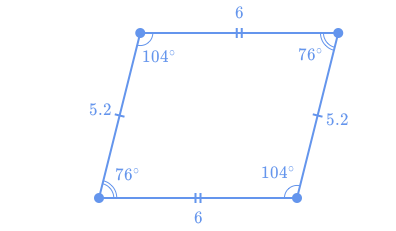
\includegraphics[scale=\shrinkfactor]{figures/8afb4df19c54a48ccc70523d29d8e73dd0c29c20.png}



\medskip
\noindent
\textbf{Tags:} {\footnotesize CC.7.G.A.2, Constructing geometric figures}\\
\textbf{Version:} d1edbdff.. 2013-10-21
\smallskip\hrule





\section{\href{https://www.khanacademy.org/devadmin/content/items/x30ec3e4c19607f03}{x30ec3e4c19607f03}}

\noindent
**Draw a parallelogram with a set of $45^\circ$ angles, set of bases length $7$, and height of $5$.** 

**Is there a unique parallelogram that satisfies the given conditions?**
[[? interactive-graph 1]]

\paragraph{Ans} 

\fbox{ Yes

}

 No



\paragraph{Hint 1}A parallelogram is a quadrilateral with two sets of equal sides sides parallel each other. 

Let�s start by drawing a parallelogram with two bases of length $\blue7$ parallel to each other and a height of $\blue5$. The height is the vertical distance perpendicular to both bases.

\paragraph{Hint 2}A parallelogram has two sets of equal angles opposite each other. There is a set of acute (less than $\purple{90^\circ}$) angles and a set of obtuse angles (greater than $\purple{90^\circ}$). In general, all four angles of a quadrilateral sum to $\pink{360^\circ}$.

We have a set of acute angles $\blue{45^\circ}$. By drawing, we find a set of obtuse angles  $\blue{135^\circ}$. Our angles sum to $\pink{360^\circ}$.

\paragraph{Hint 3}Since we are given the shape is a parallelogram and know a set of angles, set of bases and height, we can draw a parallelogram of one shape and one size. 

\paragraph{Hint 4}With the given conditions, the parallelogram is unique.


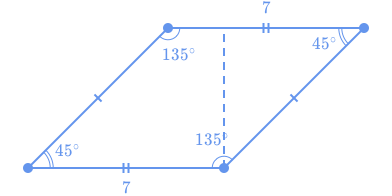
\includegraphics[scale=\shrinkfactor]{figures/bedf8aea7cdbe8811ff13c3c031c0dce292033ca.png}



\medskip
\noindent
\textbf{Tags:} {\footnotesize CC.7.G.A.2, Constructing geometric figures}\\
\textbf{Version:} 84dbc58d.. 2013-10-21
\smallskip\hrule





\section{\href{https://www.khanacademy.org/devadmin/content/items/x3813f0553f9574f3}{x3813f0553f9574f3}}

\noindent
**How many rectangles can be drawn with both diagonals length $13$?**

\paragraph{Ans} 

None

\fbox{ Only one

}

 More than one



\paragraph{Hint 1}A rectangle is a quadrilateral with four right angles and two sets of equal sides sides parallel to each other. 

Let�s start by drawing a rectangle with both diagonals of length $\blue{13}$. The diagonals of a rectangle intersect at each other at their midpoints.


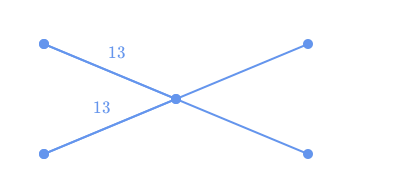
\includegraphics[scale=\shrinkfactor]{figures/ee8eceeffd155a94f3bf574f7d8664ee513f60ee.png}

\paragraph{Hint 2}Let's connect the endpoints of our diagonals to create a rectangle.


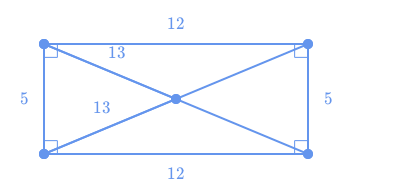
\includegraphics[scale=\shrinkfactor]{figures/6a5c37c3533378c8b4ae12c42677e1618de61f1b.png} 

\paragraph{Hint 3}Given the conditions, only one rectangle can be drawn.


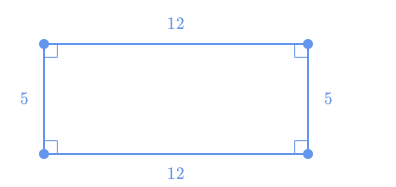
\includegraphics[scale=\shrinkfactor]{figures/83a8d869b1e347a41e5e206c6d9acf674d1e1f79.png}



\medskip
\noindent
\textbf{Tags:} {\footnotesize CC.7.G.A.2, Constructing geometric figures}\\
\textbf{Version:} 3faa1823.. 2013-10-22
\smallskip\hrule





\section{\href{https://www.khanacademy.org/devadmin/content/items/x385b2e1415652b6c}{x385b2e1415652b6c}}

\noindent
**Draw a trapezoid with $135^\circ$ and $45^\circ$ angles, two sets of perpendicular sides, and parallel bases of lengths $8$ and $14$?.**

**Is there a unique trapezoid that satisfies the given conditions?**
[[? interactive-graph 1]]

\paragraph{Ans} 

\fbox{ Yes

}

 No



\paragraph{Hint 1}Let�s start by drawing.  A trapezoid has four sides and at least one pair of parallel sides.  

Let's start by drawing a trapezoid with two sets of perpendicular sides. 


\includegraphics[scale=\shrinkfactor]{figures/75d41dbb8e47cf8e05fb47080572010c94d2ae60.png}

Next, we can adjust the length of the parallel bases to be of lengths $\blue8$ and $\blue{14}$.

\paragraph{Hint 2}Let's adjust the height of the trapezoid until we have $\blue{135^\circ}$ and $\blue{45^\circ}$ angles. The $\blue{45^\circ}$ angles must be next to the longest side length $\blue{14}$. We find the height is $\blue6$.

We can draw only one trapezoid of the given shape and size.

\paragraph{Hint 3}With the given conditions, the trapezoid is unique.


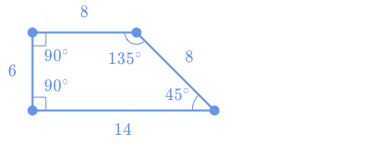
\includegraphics[scale=\shrinkfactor]{figures/3628ef704db460d85e256789062f965e0da9d254.png}



\medskip
\noindent
\textbf{Tags:} {\footnotesize CC.7.G.A.2, Constructing geometric figures}\\
\textbf{Version:} 5034b927.. 2013-10-21
\smallskip\hrule





\section{\href{https://www.khanacademy.org/devadmin/content/items/x391f877e3978e0a6}{x391f877e3978e0a6}}

\noindent
**Draw a quadrilateral with four right angles, a set of bases of length $a$, and a height of $2a$ where $a$ is any positive number.**

**Is there a unique quadrilateral that satisfies the given conditions?**
[[? interactive-graph 1]]

\paragraph{Ans} 

Yes

\fbox{ No

}

 

\paragraph{Hint 1}A quadrilateral has four straight sides and four angles. A quadrilateral with four right angles is either a square or rectangle. 

The height is drawn perpendicular to both bases. The set of bases $\blue{a}$ and a height $\blue{2a}$ are different lengths, so let's draw a rectangle. Let's choose any positive value for $\blue{a}$ and draw.

\paragraph{Hint 2}If $\blue{a}=\blue{1}$, then lets draw a rectangle with width $\blue1$ and length $\blue2$.


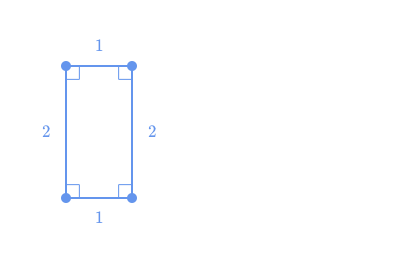
\includegraphics[scale=\shrinkfactor]{figures/08454fd7d8ef8a2085d44ab354b50ccd27560047.png}

\paragraph{Hint 3}Since $\blue{a}$ can be any positive number,  we can draw multiple rectangles given the conditions. The quadrilateral is not unique.


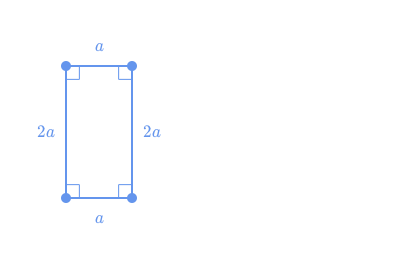
\includegraphics[scale=\shrinkfactor]{figures/082a56bb2e40ce8b302ebe6ea460056f0bfbe045.png}



\medskip
\noindent
\textbf{Tags:} {\footnotesize CC.7.G.A.2, Constructing geometric figures}\\
\textbf{Version:} cab86628.. 2013-10-21
\smallskip\hrule





\section{\href{https://www.khanacademy.org/devadmin/content/items/x3d6439a781597d9c}{x3d6439a781597d9c}}

\noindent
**How many trapezoids can be drawn with parallel bases of lengths $10$ and $5$ and a side of length $2.5$ which is perpendicular to both bases?**

\paragraph{Ans} 

None

\fbox{ Only one

}

 More than one



\paragraph{Hint 1}Let�s start by drawing.  A trapezoid has four sides and at least one pair of parallel sides.  

The side of length $\blue{2.5}$ is perpendicular to both bases, so $\blue{2.5}$ is the height.

\paragraph{Hint 2}The bases of lengths $\blue{10}$ and of length $\blue{5}$ can be drawn at a perpendicular distance of $\blue{2.5}$ to each other.

\paragraph{Hint 3}With the given conditions, we can draw only one trapezoid.
 


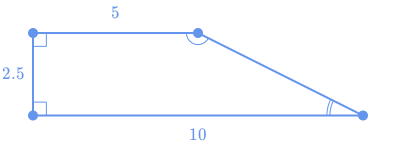
\includegraphics[scale=\shrinkfactor]{figures/338921217626d4bab40df4df3f0d95f132eb9bd4.png} 

\paragraph{Hint 4}Given the conditions, only one trapezoid can be drawn.



\medskip
\noindent
\textbf{Tags:} {\footnotesize CC.7.G.A.2, Constructing geometric figures}\\
\textbf{Version:} 036d4c6b.. 2013-10-21
\smallskip\hrule





\section{\href{https://www.khanacademy.org/devadmin/content/items/x4406265532087ad6}{x4406265532087ad6}}

\noindent
**Draw a kite with a right angle, a set of $93^\circ$ angles, and an acute angle.** 

**With these conditions, is the kite unique?**
[[? interactive-graph 1]]

\paragraph{Ans} 

Yes

\fbox{ No

}

 

\paragraph{Hint 1}A kite is a quadrilateral with four sides and four angles. A kite has two pairs of equal sides which are next to each other. 

Let's start by drawing a right $\blue{90}^\circ$ angle.

\paragraph{Hint 2}From the right angle, let's draw two sides equal in length. Then, let's form the two $\blue{93}^\circ$ angles by drawing an acute angle opposite the $\blue{90}^\circ$ angle. 

An acute angle is less than $\blue{90}^\circ$.

\paragraph{Hint 3}We know the shape of the kite, but we do not know its size. We do not know the lengths of its sides or diagonals.

\paragraph{Hint 4}With the given conditions, the kite is not unique.


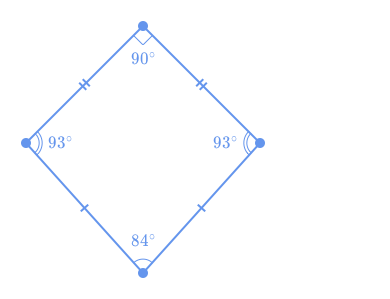
\includegraphics[scale=\shrinkfactor]{figures/124d3f2cd597ee08365d0f13074e6a525a62603e.png}



\medskip
\noindent
\textbf{Tags:} {\footnotesize CC.7.G.A.2, Constructing geometric figures}\\
\textbf{Version:} 310226be.. 2013-10-22
\smallskip\hrule





\section{\href{https://www.khanacademy.org/devadmin/content/items/x52c218226bf3c88f}{x52c218226bf3c88f}}

\noindent
**How many quadrilaterals can be drawn with all sides equal, perpendicular and of length $5$?**

\paragraph{Ans} 

None

\fbox{ Only one

}

 More than one



\paragraph{Hint 1}A quadrilateral is a plane figure with four straight sides and four angles. 

We know all four sides are equal and of length $\blue5$. Since all sides are perpendicular, we know the measures of each of the four angles to be $\blue{90^\circ}$.

Let's start by drawing.

\paragraph{Hint 2}We can draw a square with four right angles and sides $\blue5$. 

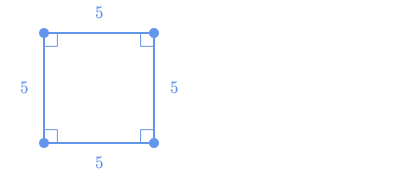
\includegraphics[scale=\shrinkfactor]{figures/526063e8cf9fd7d21cb615727f222ca592ca0cef.png} 

We can draw a square with of only one size.

\paragraph{Hint 3}Given the conditions, only one quadrilateral can be drawn.



\medskip
\noindent
\textbf{Tags:} {\footnotesize CC.7.G.A.2, Constructing geometric figures}\\
\textbf{Version:} 72b5c4ff.. 2013-10-21
\smallskip\hrule





\section{\href{https://www.khanacademy.org/devadmin/content/items/x55feedf890bb9701}{x55feedf890bb9701}}

\noindent
**Draw a rhombus with a set of $45^\circ$ angles.** 

**With these conditions, is the rhombus unique?**
[[? interactive-graph 1]]

\paragraph{Ans} 

Yes

\fbox{ No

}

 

\paragraph{Hint 1}A rhombus is a parallelogram with all sides equal. A parallelogram has four straight sides where opposite sides are parallel. 

Let�s start by drawing a rhombus with a set of $\blue{45^\circ}$ angles.

\paragraph{Hint 2}A parallelogram has a set of acute angles (less than $\purple{90^\circ}$) and a set of obtuse angles (greater than $\purple{90^\circ}$). In general, all four angles of a parallelogram sum to $\pink{360^\circ}$. 

We are given a set of acute angles $\blue{45^\circ}$. By drawing we can find the measure of the set of obtuse angles $\blue{135^\circ}$. All four angles sum to $\pink{360^\circ}$.

\paragraph{Hint 3}Since we know only the measures of the four angles and do not know the measures of the four sides, we can draw more than one rhombus of the same shape but different size.

\paragraph{Hint 4}With the given conditions, the rhombus is not unique.


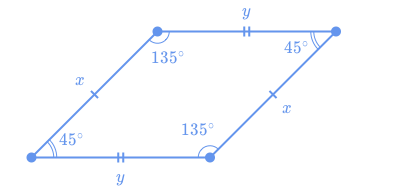
\includegraphics[scale=\shrinkfactor]{figures/4286bb81215b04f62ce80ef20a85ac55748b840f.png}



\medskip
\noindent
\textbf{Tags:} {\footnotesize CC.7.G.A.2, Constructing geometric figures}\\
\textbf{Version:} 3927af58.. 2013-10-21
\smallskip\hrule





\section{\href{https://www.khanacademy.org/devadmin/content/items/x5c7e8049b9672507}{x5c7e8049b9672507}}

\noindent
**How many quadrilaterals can be drawn with two right angles, only one set of parallel sides and two sets of perpendicular sides?**

\paragraph{Ans} 

None

Only one

\fbox{ More than one

}

 

\paragraph{Hint 1}A quadrilateral is a plane figure with four straight sides and four angles. Right angles are $\blue{{90}^\circ}$ angles. Parallel sides are an equal distant apart at every point.

Let's start by drawing two right angles:



\includegraphics[scale=\shrinkfactor]{figures/038aa61abbe40ecb60d27a9a57d975d1b6d692de.png}

We now have two sets of perpendicular sides and one set of parallel lines.

\paragraph{Hint 2}We can only have one set of parallel lines, so we increase the length of one of the perpendicular sides.



\includegraphics[scale=\shrinkfactor]{figures/0b5b4528247f0abda6afeb27054115dff1f6472e.png} 

\paragraph{Hint 3}Let's close the figure to make a quadrilateral with four straight sides. We have a trapezoid.



\includegraphics[scale=\shrinkfactor]{figures/fdda0c77898ea7407a2a95429900dc2d1fafc13e.png}

We are not given any measures of sides or the other angles. We can draw many trapezoids of different shapes and sizes.

\paragraph{Hint 4}Given the conditions, more than one quadrilateral can be drawn.



\medskip
\noindent
\textbf{Tags:} {\footnotesize CC.7.G.A.2, Constructing geometric figures}\\
\textbf{Version:} 082adffa.. 2013-10-21
\smallskip\hrule





\section{\href{https://www.khanacademy.org/devadmin/content/items/x636b464bfdbdef50}{x636b464bfdbdef50}}

\noindent
**How many quadrilaterals can be drawn with two sides of length $5$ and two sides of length $15$?**

\paragraph{Ans} 

None

Only one

\fbox{ More than one

}

 

\paragraph{Hint 1}A quadrilateral is a plane figure with four straight sides and four angles. 

Two sides are of length $\blue5$, and the other two sides are of length $\blue4$.  Let's start by drawing.

\paragraph{Hint 2}We can draw a rectangle.
. 

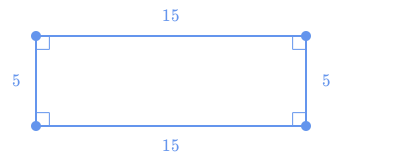
\includegraphics[scale=\shrinkfactor]{figures/1b23f020af34fcb1f911ebd94130503b9ff239ea.png} 

We cannot draw any other size rectangle. Can we draw any other shape?

\paragraph{Hint 3}We can draw a kite.


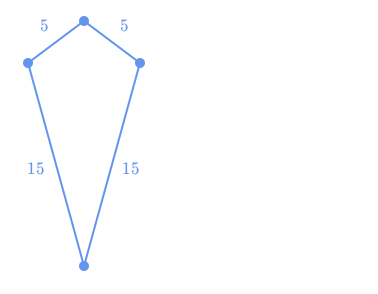
\includegraphics[scale=\shrinkfactor]{figures/3f7d7ef95693695db4029c4091822bbcdd3ac71c.png}

We can also draw a parallelogram. Since we are not given any measures of angles, so we can draw at least two quadrilaterals of different shapes and sizes.

\paragraph{Hint 4}Given the conditions, more than one quadrilateral can be drawn.



\medskip
\noindent
\textbf{Tags:} {\footnotesize CC.7.G.A.2, Constructing geometric figures}\\
\textbf{Version:} 12c768ba.. 2013-10-21
\smallskip\hrule





\section{\href{https://www.khanacademy.org/devadmin/content/items/x6cc102bdc03ffd69}{x6cc102bdc03ffd69}}

\noindent
**Draw a quadrilateral with four right angles, a set of bases of length $6.5$, and a height of $12.5$.**

**Is there a unique quadrilateral that satisfies the given conditions?**
[[? interactive-graph 1]]

\paragraph{Ans} 

\fbox{ Yes

}

 No



\paragraph{Hint 1}Let�s start by drawing. A quadrilateral has four straight sides and four angles. A quadrilateral with four right angles is either a square or rectangle. The height is drawn perpendicular to both bases.

\paragraph{Hint 2}We have a set of bases and a height of different lengths, so we draw a rectangle with side lengths $\blue{6.5}$ and $\blue{12.5}$. 

\paragraph{Hint 3}We can draw only one rectangle of the given shape and size. With the given conditions, the quadrilateral is unique.


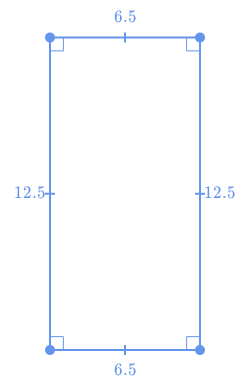
\includegraphics[scale=\shrinkfactor]{figures/fc99b93761477f7ea295fe00e72af1e7d02b6de1.png}



\medskip
\noindent
\textbf{Tags:} {\footnotesize CC.7.G.A.2, Constructing geometric figures}\\
\textbf{Version:} 4c371c90.. 2013-10-21
\smallskip\hrule





\section{\href{https://www.khanacademy.org/devadmin/content/items/x716a1fba964f151d}{x716a1fba964f151d}}

\noindent
**How many quadrilaterals can be drawn with two sets of parallel sides, a set of sides length $5$ and a set of sides length $8$?**

\paragraph{Ans} 

None

Only one

\fbox{ More than one

}

 

\paragraph{Hint 1}A quadrilateral is a plane figure with four straight sides and four angles. 

Two sides are of length $\blue5$, and the other two sides are of length $\blue8$. Let's start by drawing.

\paragraph{Hint 2}We can draw a rectangle with two sets of parallel sides, a sets of sides length $\blue5$ and a set of sides length $\blue8$. Parallel sides are an equal distance apart at every point.
. 

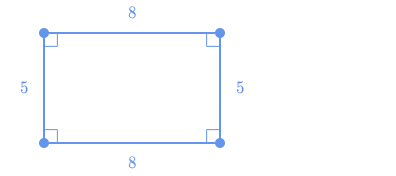
\includegraphics[scale=\shrinkfactor]{figures/02e7aa710265fc5cf3fe5914f166fcbb5989408f.png} 

We cannot draw any other size rectangle. Can we draw any other shape?

\paragraph{Hint 3}We can draw a parallelogram with the same conditions but different angles.


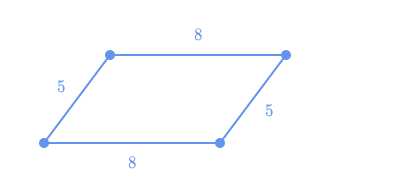
\includegraphics[scale=\shrinkfactor]{figures/937fef79524925ea6841e5bfc58a5317553626ae.png}

Since we are not given any measures of angles, so we can draw more than one quadrilateral of different shapes and sizes.

\paragraph{Hint 4}Given the conditions, more than one quadrilateral can be drawn.



\medskip
\noindent
\textbf{Tags:} {\footnotesize CC.7.G.A.2, Constructing geometric figures}\\
\textbf{Version:} a6b82ca1.. 2013-10-21
\smallskip\hrule





\section{\href{https://www.khanacademy.org/devadmin/content/items/x8344c3a5d9d93169}{x8344c3a5d9d93169}}

\noindent
**How many parallelograms can be drawn with a set of  $120^\circ$ angles and a set $90^\circ$ angles?**

\paragraph{Ans} 

\fbox{ None

}

 Only one

More than one



\paragraph{Hint 1}A parallelogram is quadrilateral with two pairs of parallel and equal sides. 

A parallelogram has two sets of equal angles opposite each other. There is a set of acute (less than $\purple{90^\circ}$) angles and a set of obtuse angles (greater than $\purple{90^\circ}$). In general, all four angles of a quadrilateral sum to $\pink{360^\circ}$.

Let's start by drawing.

\paragraph{Hint 2}If a parallelogram has only a set of $\blue{90^\circ}$ angles, then the remaining set of angles must be $\blue{90^\circ}$ as well to sum to $\pink{360^\circ}$. In this case, our parallelogram would be a rectangle or square and could not have a set of obtuse angles.


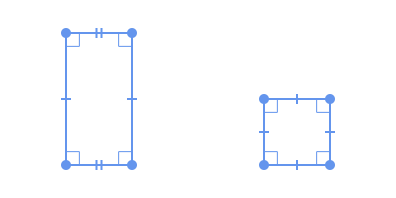
\includegraphics[scale=\shrinkfactor]{figures/890ee06a7a90e9a2c1da7b351bb293d8a07bc82a.png}

\paragraph{Hint 3}Given the conditions, no quadrilaterals can be drawn.



\medskip
\noindent
\textbf{Tags:} {\footnotesize CC.7.G.A.2, Constructing geometric figures}\\
\textbf{Version:} 6410afa1.. 2013-10-21
\smallskip\hrule





\section{\href{https://www.khanacademy.org/devadmin/content/items/x8b85f66442829666}{x8b85f66442829666}}

\noindent
**How many kites can be drawn with a set of sides length $5$ and a set of sides length $15$?**

\paragraph{Ans} 

None

\fbox{ Only one

}

 More than one



\paragraph{Hint 1}A kite is a quadrilateral and has two pairs of equal sides which are next to each other.

Let�s start by drawing. The sides of length $\blue{5}$ are next to each other. The sides of length $\blue{15}$ are next to each other.

\paragraph{Hint 2}Since we are given the shape and the size of the kite, we can draw only one kite.


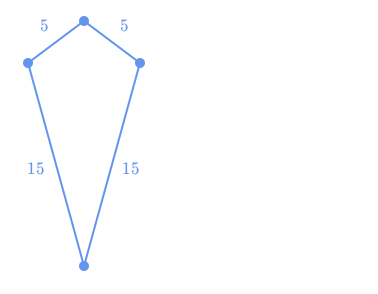
\includegraphics[scale=\shrinkfactor]{figures/3f7d7ef95693695db4029c4091822bbcdd3ac71c.png}



\medskip
\noindent
\textbf{Tags:} {\footnotesize CC.7.G.A.2, Constructing geometric figures}\\
\textbf{Version:} 191253c9.. 2013-10-22
\smallskip\hrule





\section{\href{https://www.khanacademy.org/devadmin/content/items/x95415aebb943b231}{x95415aebb943b231}}

\noindent
**Draw a trapezoid with parallel bases of lengths $15$ and $6$ and a side of length $13$ which is perpendicular to both bases.** 

**Is there a unique trapezoid that satisfies the given conditions?**
[[? interactive-graph 1]]

\paragraph{Ans} 

\fbox{ Yes

}

 No



\paragraph{Hint 1}Let�s start by drawing.  A trapezoid has four sides and at least one pair of parallel sides.  

The side of length $\blue{13}$ is perpendicular to both bases, so $\blue{13}$ is the height.

\paragraph{Hint 2}The bases of lengths $\blue{6}$ and of length $\blue{15}$ can be drawn at a perpendicular distance of $\blue{13}$.

We can draw only one trapezoid.

\paragraph{Hint 3}With the given conditions, the trapezoid is unique.

 
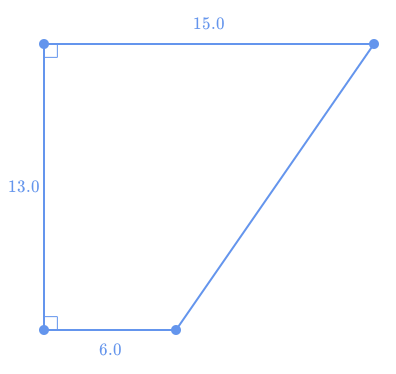
\includegraphics[scale=\shrinkfactor]{figures/13657be9021ee045c589a2d3ae1fabdc5792db54.png}



\medskip
\noindent
\textbf{Tags:} {\footnotesize CC.7.G.A.2, Constructing geometric figures}\\
\textbf{Version:} b4c8f968.. 2013-10-21
\smallskip\hrule





\section{\href{https://www.khanacademy.org/devadmin/content/items/x9ea8e27d6bebc72a}{x9ea8e27d6bebc72a}}

\noindent
**Draw  an isosceles trapezoid with parallel bases of lengths $22$ and $10$ and height of $8$.**

**Is there a unique isosceles trapezoid that satisfies the given conditions?**
[[? interactive-graph 1]]

\paragraph{Ans} 

\fbox{ Yes

}

 No



\paragraph{Hint 1}Let�s start by drawing. An isosceles trapezoid has four sides with two parallel sides and two nonparallel sides equal in length.

\paragraph{Hint 2}The bases of lengths $\blue{22}$ and $\blue{10}$ are parallel to each other and set apart at a height of $\blue{8}$. The other two nonparallel sides are equal in length.

We can draw only one trapezoid.

\paragraph{Hint 3}With the given conditions, the isosceles trapezoid is unique.


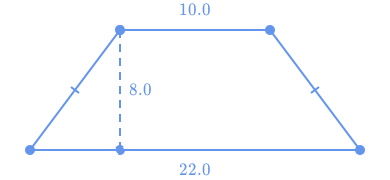
\includegraphics[scale=\shrinkfactor]{figures/7883b1f2f56b75f9e0ef790c5519e6f509573fee.png}



\medskip
\noindent
\textbf{Tags:} {\footnotesize CC.7.G.A.2, Constructing geometric figures}\\
\textbf{Version:} 2ef6ef7c.. 2013-10-21
\smallskip\hrule





\section{\href{https://www.khanacademy.org/devadmin/content/items/x9f11f9ed9a3ce004}{x9f11f9ed9a3ce004}}

\noindent
**How many parallelograms can be drawn with a set of $45^\circ$ angles, bases of length $3$ and a height of length $1$?**

\paragraph{Ans} 

None

\fbox{ Only one

}

 More than one



\paragraph{Hint 1}A parallelogram is a quadrilateral with two sets of equal sides sides parallel each other. 

Let�s start by drawing a parallelogram with two bases of length $\blue3$ parallel to each other and a height of $\blue1$. The height is the vertical distance perpendicular to both bases.

\paragraph{Hint 2}A parallelogram has two sets of equal angles opposite each other. There is a set of acute (less than $\purple{90^\circ}$) angles and a set of obtuse angles (greater than $\purple{90^\circ}$). In general, all four angles of a quadrilateral sum to $\pink{360^\circ}$.

We have a set of acute angles $\blue{45^\circ}$. By drawing, we find a set of obtuse angles  $\blue{135^\circ}$. Our angles sum to $\pink{360^\circ}$.

\paragraph{Hint 3}Since we are given the shape is a parallelogram and know a set of angles, set of bases and height, we can draw a parallelogram of one shape and one size. 


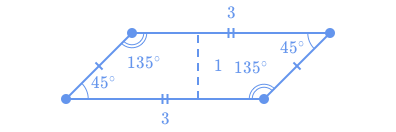
\includegraphics[scale=\shrinkfactor]{figures/c40f6c80ac7227a6193d5f0f71f72b2ebd5285aa.png} 

\paragraph{Hint 4}Given the conditions, only one parallelogram can be drawn.



\medskip
\noindent
\textbf{Tags:} {\footnotesize CC.7.G.A.2, Constructing geometric figures}\\
\textbf{Version:} 72955a42.. 2013-10-21
\smallskip\hrule





\section{\href{https://www.khanacademy.org/devadmin/content/items/xa032b60eb9810f30}{xa032b60eb9810f30}}

\noindent
**How many quadrilaterals can be drawn with four right angles and a set of sides length $5$?**

\paragraph{Ans} 

None

Only one

\fbox{ More than one

}

 

\paragraph{Hint 1}A quadrilateral is a plane figure with four straight sides and four angles. 

We are given four right angles, so we can draw either a rectangle or a square.

\paragraph{Hint 2}A set of sides is length $\blue5$. The length of the other two sides is unknown. We can draw a square with all sides length $\blue5$. 

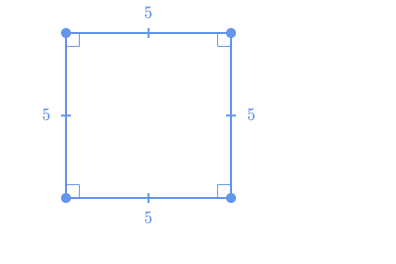
\includegraphics[scale=\shrinkfactor]{figures/f01a7ac0b5a47c41c03d6609f8ba8c6e24144389.png} 

We cannot draw any other size square. Can we draw any other shape?

\paragraph{Hint 3}We can draw many rectangles.


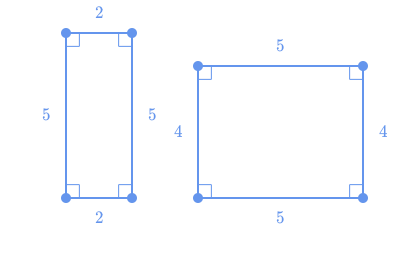
\includegraphics[scale=\shrinkfactor]{figures/7927be933ad149d8dd41e876ffe45fbdb4998383.png}

Since we are not given the measure of the other two sides, we can draw many quadrilaterals of different shapes and sizes.

\paragraph{Hint 4}Given the conditions, more than one quadrilateral can be drawn.



\medskip
\noindent
\textbf{Tags:} {\footnotesize CC.7.G.A.2, Constructing geometric figures}\\
\textbf{Version:} 52b1c16e.. 2013-10-21
\smallskip\hrule





\section{\href{https://www.khanacademy.org/devadmin/content/items/xa21aff95ae1f9a2c}{xa21aff95ae1f9a2c}}

\noindent
**How many quadrilaterals can be drawn with four right angles and side lengths $5$, $7$, $5$, and $9$?**

\paragraph{Ans} 

\fbox{ None

}

 Only one

More than one



\paragraph{Hint 1}A quadrilateral is a plane figure with four straight sides and four angles. We are given four right angles, so we can try to draw only a rectangle.

\paragraph{Hint 2}A rectangle has two sets of equal sides. We only have one set of equal sides of length $\blue{5}$. The other two sides of lengths $\blue{7}$ and $\blue{9}$ are not equal.


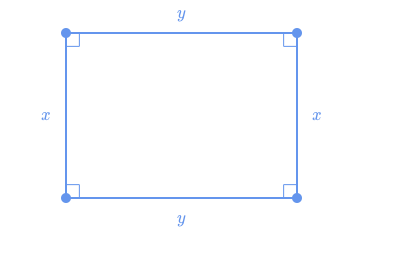
\includegraphics[scale=\shrinkfactor]{figures/3c45bf0ce72b9f301c1fbae2332cba01f0a0be14.png}

\paragraph{Hint 3}Given the conditions, no quadrilateral can be drawn.



\medskip
\noindent
\textbf{Tags:} {\footnotesize CC.7.G.A.2, Constructing geometric figures}\\
\textbf{Version:} afebeb6f.. 2013-10-21
\smallskip\hrule





\section{\href{https://www.khanacademy.org/devadmin/content/items/xb3ca82bb1be672ae}{xb3ca82bb1be672ae}}

\noindent
**How many parallelograms can be drawn with a set of sides length $3$, a set of sides length $6$ and only one set of perpendicular sides?**

\paragraph{Ans} 

\fbox{ None

}

 Only one

More than one



\paragraph{Hint 1}A parallelogram is quadrilateral with two pairs of parallel and equal sides. We know the two pairs of parallel sides are of lengths $\blue3$ and $\blue6$. 

Let's try to draw a parallelogram with only one set of perpendicular sides.

\paragraph{Hint 2}A parallelogram has two sets of equal angles. There is a set of acute (less than $\purple{90^\circ}$) angles and a set of obtuse angles (greater than $\purple{90^\circ}$). In general, any quadrilateral has $\pink{360^\circ}$ total.

If a parallelogram has only one set of perpendicular (or $\purple{90^\circ}$) sides, then the remaining sides must be $\purple{90^\circ}$ as well.

\paragraph{Hint 3}If our parallelogram were a rectangle, then it cannot have only one set of perpendicular sides. A rectangle has two sets of perpendicular sides.

\paragraph{Hint 4}Given the conditions, no quadrilaterals can be drawn.



\medskip
\noindent
\textbf{Tags:} {\footnotesize CC.7.G.A.2, Constructing geometric figures}\\
\textbf{Version:} c7f872f0.. 2013-10-21
\smallskip\hrule





\section{\href{https://www.khanacademy.org/devadmin/content/items/xbad736895bc61bbf}{xbad736895bc61bbf}}

\noindent
**Draw a quadrilateral with four right angles, a set of sides length $4$ and a set of sides length $13$.**

**Is there a unique quadrilateral that satisfies the given conditions?**
[[? interactive-graph 1]]

\paragraph{Ans} 

\fbox{ Yes

}

 No



\paragraph{Hint 1}Let�s start by drawing. A quadrilateral has four straight sides and four angles. A quadrilateral with four right angles is either a square or rectangle. 

\paragraph{Hint 2}We have two sets of sides of different lengths, so we draw a rectangle with side lengths $\blue4$ and $\blue{13}$. 

\paragraph{Hint 3}We can draw only one rectangle of the given shape and size. With the given conditions, the quadrilateral is unique.


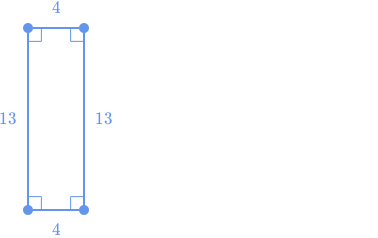
\includegraphics[scale=\shrinkfactor]{figures/19a22104b2f6226d2415d0f4aef57ae90d3f801f.png}



\medskip
\noindent
\textbf{Tags:} {\footnotesize CC.7.G.A.2, Constructing geometric figures}\\
\textbf{Version:} 92a2dd78.. 2013-10-21
\smallskip\hrule





\section{\href{https://www.khanacademy.org/devadmin/content/items/xbd5b3a895f08e909}{xbd5b3a895f08e909}}

\noindent
**Draw a quadrilateral with equal diagonals and equal side lengths.**

**Is there a unique quadrilateral that satisfies the given conditions?**
[[? interactive-graph 1]]

\paragraph{Ans} 

Yes

\fbox{ No

}

 

\paragraph{Hint 1}A quadrilateral has four straight sides and four angles. Let's start by drawing a quadrilateral with equal sides.

\paragraph{Hint 2}Since the diagonals are equal, we draw a square.

We have do not know the side length of our drawing, so we can draw many squares.

\paragraph{Hint 3}With the given conditions, the quadrilateral is not unique.


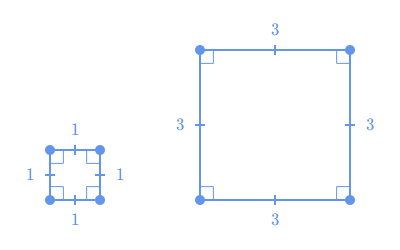
\includegraphics[scale=\shrinkfactor]{figures/d1d990fb2d10789904a7314fcc4b534710bfbf28.png}



\medskip
\noindent
\textbf{Tags:} {\footnotesize CC.7.G.A.2, Constructing geometric figures}\\
\textbf{Version:} b027026b.. 2013-10-21
\smallskip\hrule





\section{\href{https://www.khanacademy.org/devadmin/content/items/xc1b95b3889da52e2}{xc1b95b3889da52e2}}

\noindent
**Draw a rhombus with sides length $8.5$ and a set of $45^\circ$ angles.** 

**With these conditions, is the rhombus unique?**
[[? interactive-graph 1]]

\paragraph{Ans} 

\fbox{ Yes

}

 No



\paragraph{Hint 1}A rhombus is a parallelogram with all sides equal. A parallelogram has four straight sides where opposite sides are parallel. 

Let�s start by drawing a rhombus with all four sides equal to $\blue{8.5}$.

\paragraph{Hint 2}A parallelogram has a set of acute angles (less than $\purple{90^\circ}$) and a set of obtuse angles (greater than $\purple{90^\circ}$). In general, all four angles of a parallelogram sum to $\pink{360^\circ}$. 

\paragraph{Hint 3}We are given a set of acute angles $\blue{45^\circ}$. By drawing we can find the measure of the set of obtuse angles $\blue{135^\circ}$. All four angles sum to $\pink{360^\circ}$.

\paragraph{Hint 4}Since we know only the measures of the four angles and four sides, we can draw one rhombus of a unique size and shape.

\paragraph{Hint 5}With the given conditions, the rhombus is unique.


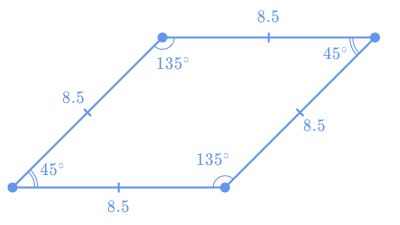
\includegraphics[scale=\shrinkfactor]{figures/a4b9805578beb58202c2f2d8440499cdd1f6547d.png}



\medskip
\noindent
\textbf{Tags:} {\footnotesize CC.7.G.A.2, Constructing geometric figures}\\
\textbf{Version:} 0f4dd958.. 2013-10-21
\smallskip\hrule





\section{\href{https://www.khanacademy.org/devadmin/content/items/xc2f881305c00d34e}{xc2f881305c00d34e}}

\noindent
**How many quadrilaterals can be drawn with all sides equal, parallel and of length $5$?**

\paragraph{Ans} 

None

Only one

\fbox{ More than one

}

 

\paragraph{Hint 1}A quadrilateral is a plane figure with four straight sides and four angles. 

We know all four sides are equal, parallel and of length $\blue5$. We do not know the measures of the $4$ angles. Let's start by drawing.

\paragraph{Hint 2}We can draw a square with four right angles and sides equal, parallel and of length $\blue5$. 

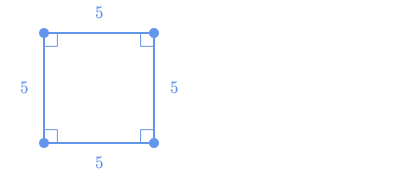
\includegraphics[scale=\shrinkfactor]{figures/526063e8cf9fd7d21cb615727f222ca592ca0cef.png} 

We cannot draw any other size square given the conditions. Can we draw any other shape?

\paragraph{Hint 3}We are not given any measures of angles, so we can draw a rhombus with sides $\blue5$ where all sides are equal and parallel as well.


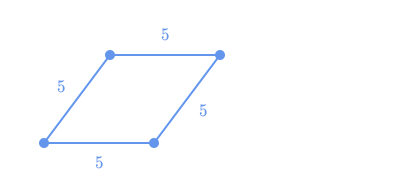
\includegraphics[scale=\shrinkfactor]{figures/4a9fd8f9c49d9b9fbaf515c2c3b2c3cde439dc8f.png}

\paragraph{Hint 4}Given the conditions, more than one quadrilateral can be drawn.



\medskip
\noindent
\textbf{Tags:} {\footnotesize CC.7.G.A.2, Constructing geometric figures}\\
\textbf{Version:} a539f8f5.. 2013-10-21
\smallskip\hrule





\section{\href{https://www.khanacademy.org/devadmin/content/items/xc558f7a2154c4fee}{xc558f7a2154c4fee}}

\noindent
**Draw a quadrilateral with only one set of parallel bases of lengths $a$ and $2a$, two sets of perpendicular sides, and a height of $a$ where $a$ is any positive number?**

**Is there a unique quadrilateral that satisfies the given conditions?**
[[? interactive-graph 1]]

\paragraph{Ans} 

Yes

\fbox{ No

}

 

\paragraph{Hint 1}A quadrilateral is a plane figure with four straight sides and four angles. Right angles are $\blue{{90}^\circ}$ angles. Parallel sides are an equal distant apart at every point.

The height  $\blue{a}$ is drawn perpendicular to both bases of length  $\blue{a}$ and  $\blue{2a}$. Let's choose any positive value for $\blue{a}$ and draw.

\paragraph{Hint 2}If $\blue{a}=\blue{1}$, then lets draw parallel bases of length $\blue1$ and length $\blue2$. The height $\blue1$ is perpendicular to both bases.


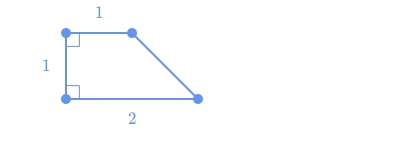
\includegraphics[scale=\shrinkfactor]{figures/48978b9582b9cb999d186b116923d62ea73d467a.png}

We now have two sets of perpendicular sides and one set of parallel lines.

\paragraph{Hint 3}Since $\blue{a}$ can be any positive number,  we can draw multiple trapezoids given the conditions. The quadrilateral is not unique.


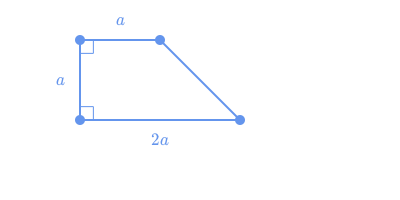
\includegraphics[scale=\shrinkfactor]{figures/08c2af6ddd19e767a58af9af63d7b3aa920dbc4a.png}



\medskip
\noindent
\textbf{Tags:} {\footnotesize CC.7.G.A.2, Constructing geometric figures}\\
\textbf{Version:} 9bccfbd4.. 2013-10-22
\smallskip\hrule





\section{\href{https://www.khanacademy.org/devadmin/content/items/xfeff8bca2ee797c6}{xfeff8bca2ee797c6}}

\noindent
**Draw a parallelogram with right angles and sides $a$ and $3a$ where $a$ is any positive number.** 

**With these conditions, is the parallelogram unique?**
[[? interactive-graph 1]]

\paragraph{Ans} 

Yes

\fbox{ No

}

 

\paragraph{Hint 1}A parallelogram is a quadrilateral with two sets of equal sides sides parallel each other. 

Let's choose any positive value for $\blue{a}$ and draw a parallelgram given the conditions.

\paragraph{Hint 2}Let�s start by drawing a parallelogram with all right angles. In other words, let's draw a rectangle.

If $\blue{a}=\blue{3}$, then lets draw parallel bases of length $\blue3$ and length $\blue{9}$.


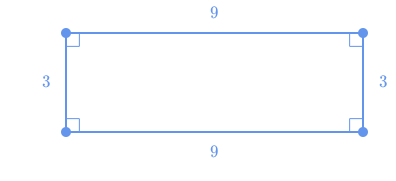
\includegraphics[scale=\shrinkfactor]{figures/01121fbdc22f76a9c7b5573e922a7445126cc90a.png}

\paragraph{Hint 3}We can choose any positive value for $\blue{a}$. We can draw more than one parallelogram of same shape but different size.

\paragraph{Hint 4}With the given conditions, the parallelogram is not unique.


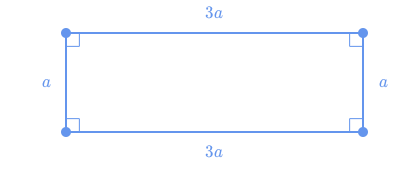
\includegraphics[scale=\shrinkfactor]{figures/1a9e466508cc481045a8490d858c74b886b844e8.png}



\medskip
\noindent
\textbf{Tags:} {\footnotesize CC.7.G.A.2, Constructing geometric figures}\\
\textbf{Version:} f8a9aeed.. 2013-10-22
\smallskip\hrule



%%  Create a directory called 'figures' in latex dir and run the following command 
%  wget -N \
%    https://ka-perseus-graphie.s3.amazonaws.com/3fcc8a0717d83f7b047263027d42633407987b91.png \
%    https://ka-perseus-graphie.s3.amazonaws.com/3fc1a3de04ae5beee01136dbc98446947a8f58f8.png \
%    https://ka-perseus-graphie.s3.amazonaws.com/249bf35a334a6b61176c6935259fb138330fc7bb.png \
%    https://ka-perseus-graphie.s3.amazonaws.com/8afb4df19c54a48ccc70523d29d8e73dd0c29c20.png \
%    https://ka-perseus-graphie.s3.amazonaws.com/bedf8aea7cdbe8811ff13c3c031c0dce292033ca.png \
%    https://ka-perseus-graphie.s3.amazonaws.com/ee8eceeffd155a94f3bf574f7d8664ee513f60ee.png \
%    https://ka-perseus-graphie.s3.amazonaws.com/6a5c37c3533378c8b4ae12c42677e1618de61f1b.png \
%    https://ka-perseus-graphie.s3.amazonaws.com/83a8d869b1e347a41e5e206c6d9acf674d1e1f79.png \
%    https://ka-perseus-graphie.s3.amazonaws.com/75d41dbb8e47cf8e05fb47080572010c94d2ae60.png \
%    https://ka-perseus-graphie.s3.amazonaws.com/3628ef704db460d85e256789062f965e0da9d254.png \
%    https://ka-perseus-graphie.s3.amazonaws.com/08454fd7d8ef8a2085d44ab354b50ccd27560047.png \
%    https://ka-perseus-graphie.s3.amazonaws.com/082a56bb2e40ce8b302ebe6ea460056f0bfbe045.png \
%    https://ka-perseus-graphie.s3.amazonaws.com/338921217626d4bab40df4df3f0d95f132eb9bd4.png \
%    https://ka-perseus-graphie.s3.amazonaws.com/124d3f2cd597ee08365d0f13074e6a525a62603e.png \
%    https://ka-perseus-graphie.s3.amazonaws.com/526063e8cf9fd7d21cb615727f222ca592ca0cef.png \
%    https://ka-perseus-graphie.s3.amazonaws.com/4286bb81215b04f62ce80ef20a85ac55748b840f.png \
%    https://ka-perseus-graphie.s3.amazonaws.com/038aa61abbe40ecb60d27a9a57d975d1b6d692de.png \
%    https://ka-perseus-graphie.s3.amazonaws.com/0b5b4528247f0abda6afeb27054115dff1f6472e.png \
%    https://ka-perseus-graphie.s3.amazonaws.com/fdda0c77898ea7407a2a95429900dc2d1fafc13e.png \
%    https://ka-perseus-graphie.s3.amazonaws.com/1b23f020af34fcb1f911ebd94130503b9ff239ea.png \
%    https://ka-perseus-graphie.s3.amazonaws.com/3f7d7ef95693695db4029c4091822bbcdd3ac71c.png \
%    https://ka-perseus-graphie.s3.amazonaws.com/fc99b93761477f7ea295fe00e72af1e7d02b6de1.png \
%    https://ka-perseus-graphie.s3.amazonaws.com/02e7aa710265fc5cf3fe5914f166fcbb5989408f.png \
%    https://ka-perseus-graphie.s3.amazonaws.com/937fef79524925ea6841e5bfc58a5317553626ae.png \
%    https://ka-perseus-graphie.s3.amazonaws.com/890ee06a7a90e9a2c1da7b351bb293d8a07bc82a.png \
%    https://ka-perseus-graphie.s3.amazonaws.com/13657be9021ee045c589a2d3ae1fabdc5792db54.png \
%    https://ka-perseus-graphie.s3.amazonaws.com/7883b1f2f56b75f9e0ef790c5519e6f509573fee.png \
%    https://ka-perseus-graphie.s3.amazonaws.com/c40f6c80ac7227a6193d5f0f71f72b2ebd5285aa.png \
%    https://ka-perseus-graphie.s3.amazonaws.com/f01a7ac0b5a47c41c03d6609f8ba8c6e24144389.png \
%    https://ka-perseus-graphie.s3.amazonaws.com/7927be933ad149d8dd41e876ffe45fbdb4998383.png \
%    https://ka-perseus-graphie.s3.amazonaws.com/3c45bf0ce72b9f301c1fbae2332cba01f0a0be14.png \
%    https://ka-perseus-graphie.s3.amazonaws.com/19a22104b2f6226d2415d0f4aef57ae90d3f801f.png \
%    https://ka-perseus-graphie.s3.amazonaws.com/d1d990fb2d10789904a7314fcc4b534710bfbf28.png \
%    https://ka-perseus-graphie.s3.amazonaws.com/a4b9805578beb58202c2f2d8440499cdd1f6547d.png \
%    https://ka-perseus-graphie.s3.amazonaws.com/4a9fd8f9c49d9b9fbaf515c2c3b2c3cde439dc8f.png \
%    https://ka-perseus-graphie.s3.amazonaws.com/48978b9582b9cb999d186b116923d62ea73d467a.png \
%    https://ka-perseus-graphie.s3.amazonaws.com/08c2af6ddd19e767a58af9af63d7b3aa920dbc4a.png \
%    https://ka-perseus-graphie.s3.amazonaws.com/01121fbdc22f76a9c7b5573e922a7445126cc90a.png \
%    https://ka-perseus-graphie.s3.amazonaws.com/1a9e466508cc481045a8490d858c74b886b844e8.png \


\end{document}